\documentclass[a4paper,11pt]{article}
\usepackage[margin=22mm]{geometry}
\usepackage[T1]{fontenc}
\usepackage[utf8]{inputenc}
\usepackage[ngerman]{babel}
\usepackage{lmodern,graphicx,booktabs,pgfplots,enumitem}
\pgfplotsset{compat=1.18}
\definecolor{ochre}{RGB}{155,112,0}
\definecolor{navy}{RGB}{36,92,170}
\definecolor{brick}{RGB}{185,56,50}
\setlength{\parindent}{0pt}
\setlength{\parskip}{4pt}
\renewcommand{\arraystretch}{1.13}
\raggedbottom
\setlist[itemize]{leftmargin=*,itemsep=2pt,topsep=4pt}
\begin{document}
\textbf{Haus: früherer Cachetest} \hfill \texttt{2026110103}

{\small Source-Stopp: 60,069 s\quad ohne Pinning\quad Empfänger: 360 s}

\begin{center}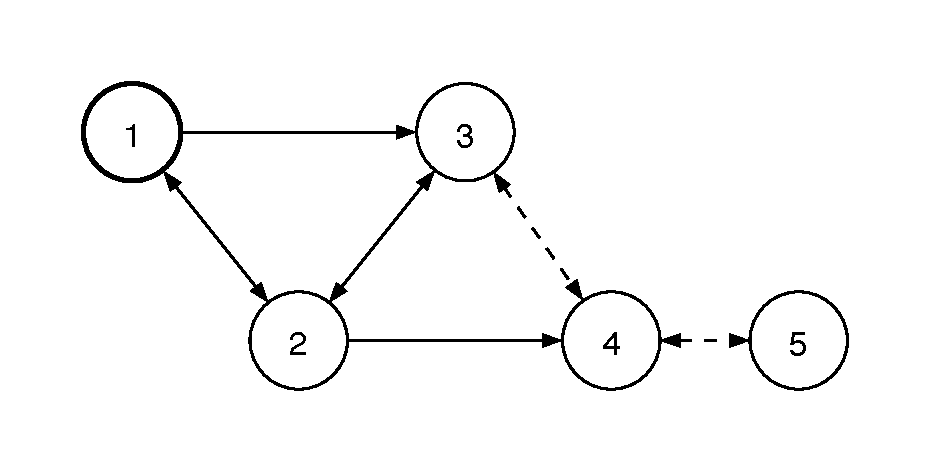
\includegraphics[width=13cm,height=4.4cm,keepaspectratio]{h2.pdf}\end{center}

{\small Pfeil: Sender $\rightarrow$ Empfänger; gesamter Lauf. Linie: Seiten; gestrichelt: nur Beacons.}

\begin{center}\small
\begin{tabular}{clcc}\toprule
Board & Gehört & Seiten & Fehlende ID \\ \midrule
1 & 2 & Quelle & -- \\
2 & 1, 3 & 5/5 & -- \\
3 & 1, 2, 4 & 5/5 & -- \\
4 & 2, 3, 5 & 2/5 & 0, 1, 2 \\
5 & 4 & 0/5 & 0, 1, 2, 3, 4 \\
\bottomrule\end{tabular}
\end{center}

\begin{center}\begin{tikzpicture}\begin{axis}[
width=16cm,height=5.8cm,xmin=0,xmax=360,ymin=-0.08,ymax=5.3,
ytick={0,1,2,3,4,5},xtick distance=60,axis lines=left,grid=major,major grid style={gray!15},
xlabel={Zeit seit lokalem Start (s)},ylabel={Verschiedene Seiten},
tick label style={font=\small},label style={font=\small},
legend style={draw=none,font=\small,at={(0.5,-0.25)},anchor=north,legend columns=4}]
\addplot[ochre,dashdotted,thick,const plot,no marks] coordinates {(0.000,0) (35.910,1) (37.952,2) (41.374,3) (71.733,4) (82.130,5) (360.000,5)};
\addlegendentry{Board 2}
\addplot[navy,solid,thick,const plot,no marks] coordinates {(0.000,0) (48.850,1) (50.893,2) (52.948,3) (94.931,4) (97.126,5) (360.000,5)};
\addlegendentry{Board 3}
\addplot[brick,dashed,thick,const plot,no marks] coordinates {(0.000,0) (75.750,1) (109.531,2) (360.000,2)};
\addlegendentry{Board 4}
\addplot[black,densely dotted,thick,const plot,no marks] coordinates {(0.000,0) (360.000,0)};
\addlegendentry{Board 5}
\end{axis}\end{tikzpicture}\end{center}

\begin{center}\small
\begin{tabular}{ccccc}\toprule
Seite & Board 2 & Board 3 & Board 4 & Board 5 \\ \midrule
0 & 41,374 (1) & 48,850 (1) & fehlt & fehlt \\
1 & 82,130 (1) & 97,126 (2) & fehlt & fehlt \\
2 & 35,910 (1) & 50,893 (1) & fehlt & fehlt \\
3 & 71,733 (1) & 94,931 (2) & 109,531 (2) & fehlt \\
4 & 37,952 (1) & 52,948 (2) & 75,750 (2) & fehlt \\
\midrule
5/5 nach & 82,130 & 97,126 & -- & -- \\
\bottomrule\end{tabular}
\end{center}

{\small Erste Ankunft in Sekunden seit dem jeweiligen Start; Absender in Klammern.}

{\small Board 5: ein Beacon von 4, keine Seiten. Gemeinsame Laufzeit nicht genau bekannt.}
\newpage
\textbf{Haus: Cachetest} \hfill \texttt{2026110601}

{\small Source-Stopp: 180,156 s\quad Relais: 900 s\quad Board 5: 300 s}

\begin{center}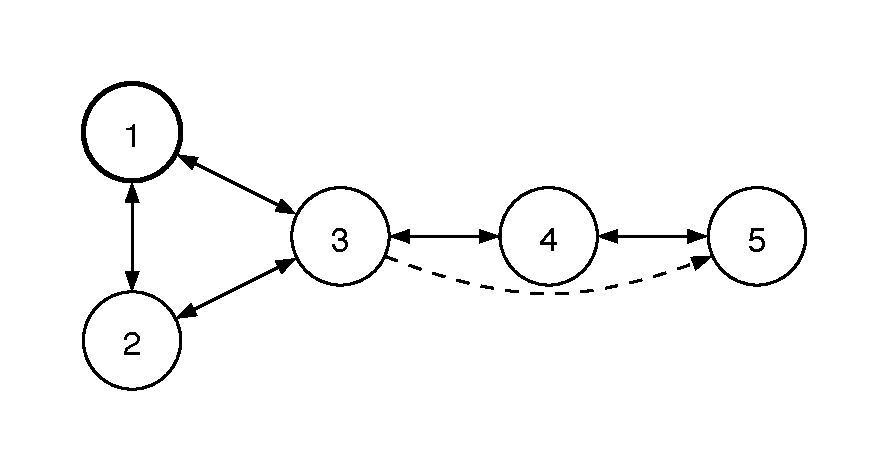
\includegraphics[width=13cm,height=4.4cm,keepaspectratio]{cache.pdf}\end{center}

{\small Pfeil: Sender $\rightarrow$ Empfänger; gesamter Lauf. Linie: Seiten; gestrichelt: nur Beacons.}

\begin{center}\small
\begin{tabular}{clcc}\toprule
Board & Gehört & Seiten & Fehlende ID \\ \midrule
1 & 2, 3 & Quelle & -- \\
2 & 1, 3 & 5/5 & -- \\
3 & 1, 2, 4 & 5/5 & -- \\
4 & 3, 5 & 4/5 & 2 \\
5 & 3, 4 & 4/5 & 2 \\
\bottomrule\end{tabular}
\end{center}

\begin{center}\begin{tikzpicture}\begin{axis}[
width=16cm,height=5.8cm,xmin=0,xmax=300,ymin=-0.08,ymax=5.3,
ytick={0,1,2,3,4,5},xtick distance=60,axis lines=left,grid=major,major grid style={gray!15},
xlabel={Zeit seit lokalem Start (s)},ylabel={Verschiedene Seiten},
tick label style={font=\small},label style={font=\small},
legend style={draw=none,font=\small,at={(0.5,-0.25)},anchor=north,legend columns=4}]
\addplot[ochre,dashdotted,thick,const plot,no marks] coordinates {(0.000,0) (74.456,1) (77.478,2) (79.272,3) (82.499,4) (92.549,5) (300.000,5)};
\addlegendentry{Board 2}
\addplot[navy,solid,thick,const plot,no marks] coordinates {(0.000,0) (89.061,1) (91.063,2) (97.105,3) (107.155,4) (110.065,5) (300.000,5)};
\addlegendentry{Board 3}
\addplot[brick,dashed,thick,const plot,no marks] coordinates {(0.000,0) (104.519,1) (135.665,2) (155.751,3) (216.003,4) (300.000,4)};
\addlegendentry{Board 4}
\addplot[black,densely dotted,thick,const plot,no marks] coordinates {(0.000,0) (5.176,1) (35.447,2) (60.170,3) (80.224,4) (300.000,4)};
\addlegendentry{Board 5}
\end{axis}\end{tikzpicture}\end{center}

\begin{center}\small
\begin{tabular}{ccccc}\toprule
Seite & Board 2 & Board 3 & Board 4 & Board 5 \\ \midrule
0 & 82,499 (1) & 97,105 (1) & 135,665 (3) & 35,447 (4) \\
1 & 74,456 (1) & 89,061 (1) & 216,003 (3) & 60,170 (4) \\
2 & 92,549 (1) & 107,155 (1) & fehlt & fehlt \\
3 & 79,272 (1) & 91,063 (1) & 104,519 (3) & 80,224 (4) \\
4 & 77,478 (1) & 110,065 (1) & 155,751 (3) & 5,176 (4) \\
\midrule
5/5 nach & 92,549 & 110,065 & -- & -- \\
Laufzeit (s) & 900,000 & 900,000 & 900,000 & 300,000 \\
\bottomrule\end{tabular}
\end{center}

{\small Diagramm: erste 300 s je Board; Starts zeitversetzt. Tabelle: Sekunden, Absender in Klammern.}

{\small Board 5: alle vier Seiten von 4. Seite 2 fehlt auch bei 4.}

{\small Während 5 lief: 3$\rightarrow$4 mit 12 Beacons, ohne Seitenframe. Relais durchgehend aktiv.}
\newpage
\textbf{Hub: Cachetest} \hfill \texttt{2026110602}

{\small Software-Stopp: 180,145 s\quad Board 5: 300 s\quad alle Boards am USB}

\begin{center}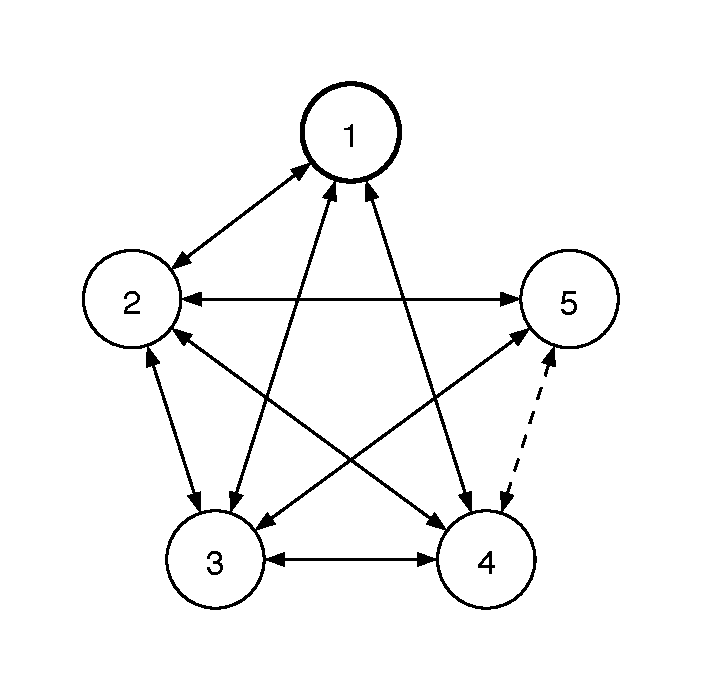
\includegraphics[width=13cm,height=4.4cm,keepaspectratio]{cachehub.pdf}\end{center}

{\small Pfeil: Sender $\rightarrow$ Empfänger; gesamter Lauf. Linie: Seiten; gestrichelt: nur Beacons.}

\begin{center}\small
\begin{tabular}{clcc}\toprule
Board & Gehört & Seiten & Fehlende ID \\ \midrule
1 & 2, 3, 4 & Quelle & -- \\
2 & 1, 3, 4, 5 & 5/5 & -- \\
3 & 1, 2, 4, 5 & 5/5 & -- \\
4 & 1, 2, 3, 5 & 5/5 & -- \\
5 & 2, 3, 4 & 5/5 & -- \\
\bottomrule\end{tabular}
\end{center}

\begin{center}\begin{tikzpicture}\begin{axis}[
width=16cm,height=5.8cm,xmin=0,xmax=300,ymin=-0.08,ymax=5.3,
ytick={0,1,2,3,4,5},xtick distance=60,axis lines=left,grid=major,major grid style={gray!15},
xlabel={Zeit seit lokalem Start (s)},ylabel={Verschiedene Seiten},
tick label style={font=\small},label style={font=\small},
legend style={draw=none,font=\small,at={(0.5,-0.25)},anchor=north,legend columns=4}]
\addplot[ochre,dashdotted,thick,const plot,no marks] coordinates {(0.000,0) (0.055,1) (2.110,2) (4.141,3) (4.667,4) (9.699,5) (300.000,5)};
\addlegendentry{Board 2}
\addplot[navy,solid,thick,const plot,no marks] coordinates {(0.000,0) (1.091,1) (2.124,2) (4.169,3) (4.636,4) (9.714,5) (300.000,5)};
\addlegendentry{Board 3}
\addplot[brick,dashed,thick,const plot,no marks] coordinates {(0.000,0) (0.085,1) (1.106,2) (2.127,3) (4.171,4) (9.729,5) (300.000,5)};
\addlegendentry{Board 4}
\addplot[black,densely dotted,thick,const plot,no marks] coordinates {(0.000,0) (49.223,1) (54.057,2) (104.457,3) (150.192,4) (175.292,5) (300.000,5)};
\addlegendentry{Board 5}
\end{axis}\end{tikzpicture}\end{center}

\begin{center}\small
\begin{tabular}{ccccc}\toprule
Seite & Board 2 & Board 3 & Board 4 & Board 5 \\ \midrule
0 & 0,055 (1) & 4,636 (2) & 0,085 (1) & 54,057 (3) \\
1 & 4,667 (3) & 1,091 (1) & 1,106 (1) & 104,457 (2) \\
2 & 2,110 (4) & 2,124 (4) & 2,127 (1) & 49,223 (2) \\
3 & 9,699 (1) & 9,714 (1) & 9,729 (1) & 150,192 (3) \\
4 & 4,141 (1) & 4,169 (2) & 4,171 (1) & 175,292 (2) \\
\midrule
5/5 nach & 9,699 & 9,714 & 9,729 & 175,292 \\
Laufzeit (s) & 526,256 & 526,519 & 527,162 & 300,000 \\
\bottomrule\end{tabular}
\end{center}

{\small Diagramm: erste 300 s je Board; Starts zeitversetzt. Tabelle: Sekunden, Absender in Klammern.}

{\small Kurven 2--4 fast gleich. Board 5: 5/5 nach 175,292 s; keine Source-Frames.}

{\small Source softwareseitig gestoppt; vor Start von 5 etwa fünf Sekunden Pause.}
\newpage\textbf{Übersicht}

\begin{center}\small
\begin{tabular}{llcccc}\toprule
Run & Aufbau & 2 & 3 & 4 & 5 \\ \midrule
2026110103 & Haus, ohne Pinning & 5/5 & 5/5 & 2/5 & 0/5 \\
2026110601 & Haus, Pin + Wiederholung & 5/5 & 5/5 & 4/5 & 4/5 \\
2026110602 & Hub, Pin + Wiederholung & 5/5 & 5/5 & 5/5 & 5/5 \\
\bottomrule\end{tabular}
\end{center}

{\small Pinning und Wiederholung betreffen die Source vor dem Stopp; eine Seite alle fünf Sekunden.}

\begin{center}\small
\begin{tabular}{lccc}\toprule
Run & Source bis Stopp (s) & Fenster bei 5 (s) & Firmware \\ \midrule
2026110103 & 60,069 & 360 & \texttt{ca6fe90} \\
2026110601 & 180,156 & 300 & \texttt{9539f99} \\
2026110602 & 180,145 & 300 & \texttt{9539f99} \\
\bottomrule\end{tabular}
\end{center}

\begin{center}\small\begin{tabular}{ccll}\toprule
Board & Farbe & MAC & Ort \\ \midrule
1 & Grün & \texttt{ac276eb0f9b4} & Laptop / Quelle \\
2 & Gelb & \texttt{ac276eb0f9fc} & Korridor \\
3 & Blau & \texttt{ac276eb0059c} & Wohnzimmer \\
4 & Rot & \texttt{ac276eafeb88} & Keller \\
5 & Weiss & \texttt{ac276eb00868} & Hobbyraum \\
\bottomrule\end{tabular}\end{center}

\textbf{Stichpunkte}

\begin{itemize}

\item Neuer Hauslauf: Seite 2 bei 2 und 3 vorhanden, bei 4 und 5 fehlend.

\item Hub: 5 empfing direkt von 2 und 3; der Weg über 4 wurde umgangen.

\item Source-Zeit, Firmware, Laufzeit und Topologie unterscheiden sich. Kein isolierter Pinningvergleich.

\item Nächster Schritt: Sendeentscheidungen loggen; danach Zehn-Minuten-Läufe vorbereiten.

\end{itemize}

\end{document}
